\documentclass[11pt]{article}
\usepackage[top=20mm,bottom=30mm,left=20mm,right=20mm]{geometry}
\usepackage[utf8]{inputenc}
\usepackage{parskip}
\usepackage{abstract}

% Biblatex
\usepackage[block=space,bibencoding=utf8,style=phys,maxbibnames=6,giveninits=true]{biblatex}
\addbibresource{../StochasticTopology.bib}

% Mathy stuff
\usepackage{physics}
\usepackage{siunitx}
\usepackage{amsmath}
\usepackage[version=4]{mhchem}

% Visual stuff
\usepackage{graphics}
\usepackage{tikz}
\usetikzlibrary{math}
\usepackage{stackengine}
\usepackage{float}

% Misc
\usepackage{hyperref}
\usepackage{cleveref}
\usepackage{lipsum}

\renewcommand{\abstractname}{}    % clear the title
\renewcommand{\absnamepos}{empty} % originally center

\setlength{\parskip}{2ex}
\setlength{\parindent}{0em}

\begin{document}
\pagenumbering{gobble}
\begin{center}
	\LARGE
	\textbf{Topological States in Out-of-Equilibrium\\Allosteric Molecular Assemblies} \\
	\vspace{0.3em}
	\normalsize
	\textit{Jan Kocka}
	\vspace{1em}
\end{center}

\begin{abstract}
	% General introduction to topology in biology/biophysics - 98 words
	Despite noisiness in the cellular environment, molecular systems show a high degree of robustness.
	A recent new direction in understanding this apparent paradox is the study of topologically protected states in stochastic systems, which robustly confine the dynamics of the system to a lower dimensional space\cite{muruganTopologicallyProtectedModes2017,tangTopologyProtectsChiral2021,soneHermitianNonHermitianTopology2024}.
    However, it is unclear what the minimal biochemical ingredients are for such states to occur.
	% Getting into the project - ~110 words
    Here we study topological features in a non-equilibrium, thermodynamically consistent model of a molecular assembly, subunits of which undergo futile cycles of conformational change and phosphorylation.
    % Such futile cycles are common in biological settings\cite{sharmaFutileCyclesEmerging2024,samoilovStochasticAmplificationSignaling2005} and can give rise to topological edge currents\cite{tangTopologyProtectsChiral2021}.
    When the subunits allosterically interact with each other we find global cycles at the scale of the assembly, analogous to topological edge currents in quantum systems.
    We map out the kinetics, energetics, and biochemical interactions necessary to obtain distinct classes of topological behaviour.
    % Results-ish ->
    Our results show that stereotyped dynamics can be a result of non-equilibrium drive only, not necessitating a specific mechanism.
    In particular, we suggest that topological states can provide a minimal description of coordination in molecular systems such as circadian clocks (e.g. KaiABC) or polymer assembly (e.g. microtubules).

\end{abstract}

\vfill
\begin{figure}[H]
	\centering
	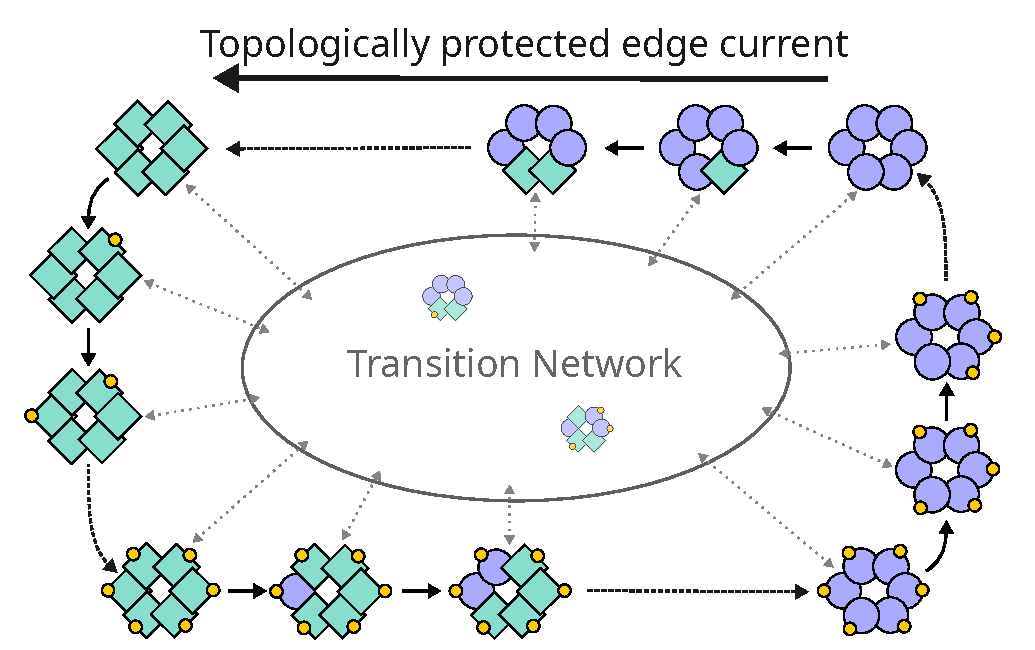
\includegraphics[width=\textwidth]{diagram/diagram_circly.pdf}
\end{figure}

\newpage
\printbibliography

\newpage
\section{New Notes}
\subsection{Questions and things to discuss}
\begin{itemize}
	\item Title! Right now it is very clunky. Should it include "thermodynamically consistent"?
    \item Conclusion bit! Very much not sure about it as it is -- is it too short? Should I specifically cite the paper I do there as that really proposes a similar but different model for it, or should I instead highlight the locality difference we add to it? Not sure
    \item In order to expand the conclusion I need to slightly cut down something.
	\item Should I reference the figure from the abstract?
	\item Little Things \begin{itemize}
		      \item Should I explicitly list what our futile cycle is? It's a bit long and perhaps obvious but I think it's nice to give a concrete, simple thing to visualize.
              \item I should probably check that using "artificially" where I do is appropriate.
              \item "this robustness" $\rightarrow$ "biological robustness"?
              \item Is "We consider" acceptable language?
	      \end{itemize}
\end{itemize}

\subsection{General}
\begin{itemize}
	\item So going for \textbf{Clocks, timers and cell cycle dynamics} topic
	\item Can I squeeze in "non-Hermitian topology" somewhere (I have some references for it, and it is relevant)?
\end{itemize}

\newpage
\section{Old Notes}
\paragraph{Format}
For POL2025 (the one due on the 6th) it should be 250 words, include references and up to 1 figure.
\paragraph{Topic}
I need to choose one of a list of topics.
Perhaps the closest might be: \textbf{"Biomolecular assemblies and condensates"} given that the main model is of an allosteric assembly?
Others that may be relevant:
\begin{itemize}
	\item "Patterns, waves, transport, collective phenomena, and microswimmers" -- there's collective phenomena! but idk about microswimmers
	\item "Clocks, timers and cell cycle dynamics" -- if we lean into KaiABC then maybe
	\item "Protein structure, dynamics and interactions" -- cause I guess the polymer as I've been calling it would realistically be a protein?
	\item "Emerging Areas in the Physics of Life" -- idk what this is but probably not
\end{itemize}

\subsection{Questions}
\begin{itemize}
	\item Approach to talk about a project that has only just started?
	\item Should I be talking about allostery or not so much? It seems relevant and as an interesting topic but it's not really a core ingredient in it.
	\item I'm a bit worried that the only "result" is a bit obvious once you think about it. If we add a penalty for NN having different conformation then of course the ones with all the same conformation will be preferred. Then if all are in conformation 1 (tense) then they are ATP driven to bind ligands so they do so. After that they are by our choice of parameters not favoured to debind hence the only thing they can do is change conformation. The same sort of reasoning then completes the cycle.
	\item Is an ArXiV citation admissible here?\cite{soneHermitianNonHermitianTopology2024}
\end{itemize}

\subsection{Key points to cover}
\begin{itemize}
	\item stochastic systems
	\item futile cycles
	\item non-equilibrium dynamics
	\item allostery
	\item system features
	      \begin{itemize}
		      \item complex -- high dimensional network, not pen-and-paper tractable
		      \item locality -- unlike the previous models, have NNs, can model waves along the polymer
		      \item discrete configurational space
		      \item Thermodynamically consistent? idk if this is the right wording
	      \end{itemize}
	\item Search for topological states/patterns in realistic systems (this means starting from the ground up with (non-equilibrium) statphys, LDB, no arbitrary choices) with futile cycles
	\item the futile cycle is implemented via physical parameters by coupling to two physically reasonable asymmetrical processes
\end{itemize}

% \subsection{"Formula"}
% \paragraph{Title/Topic}
% \paragraph{Motivation}
% Topological phases have been a hot topic in physics ever since the quantum hall effect.
% Recently their study has been extended to non-Hermitian systems such as a non-reciprocal stochastic processes.
% \paragraph{Problem}
% Idrk?
% \paragraph{Study design}
%
% \paragraph{Predictions and results}
% \paragraph{Conclusions}

\end{document}
